%!TEX root = pset2.tex

\section{Logistic Regression}\label{sec:lr}

\subsection{Implementation}
We implemented $L_2$-regularized logistic regression using gradient descent. The objective function to be minimized over is:
\begin{equation}
\sum_{i=1}^n \log (1 + e^{-y^{(i)}(\M w^T\M x^{(i)} + w_0)}) + \lambda \M w^T\M w
\end{equation}

We used both our implementation of gradient descent and the \texttt{MATLAB} function \texttt{fminunc}. Convergence criterion is reached within reasonable iterations in both implementations.

\subsection{Performance on data with $\lambda = 0$}
We run the logistic regression on the four data sets, setting the regularization parameter $\lambda = 0$. The estimated coefficients are listed in Table \ref{tab:LR_reg_coeff}.

\begin{table}[h!]
\centering
\caption{Estimated logistic regression coefficients and accuracy, $\lambda = 0$ }
\begin{tabular}{lrrrrrr}
  \hline\hline
  Data   & $w_0$ 	& $w_1$ 	  & $w_2$ 	& Train accuracy & Valid accuracy & Test accuracy\\
  \hline
  stdev1 & -66.3378  & 95.2461 & 101.1527 & 1.0000    & 1.0000    & 0.9975\\
  stdev2 & -0.0466   & 0.7636  & 1.1148 	& 0.9075    & 0.9200    & 0.9250\\
  stdev4 & -0.0093   & 0.2363  & 0.2034 	& 0.7400    & 0.7525    & 0.7825\\
  nonsep & 0.0006    & -0.0247 & -0.0237	& 0.5150    & 0.4925	   & 0.4975\\
  \hline\hline
\end{tabular}\label{tab:LR_reg_coeff}
\end{table}

The decision boundaries at various thresholds are plotted in Figure \ref{fig:LR_plots}. We observe the following phenomenon:
\begin{enumerate}
\item As data become more linearly non-separable, the accuracy is lower in all of the 
\item As data become more linearly non-separable, the estimated logistic function is also less steep, reflected in the wider bands in the plots and lower norm of $\M w$. This is reasonable because the classifier is not as certain about how to classify the data points in the mix zone.
\item In the non-separable case, logistic regression fails to classify, barely reaching the $50\%$ baseline.
\end{enumerate}


\begin{figure}[h!]
\centering
    \begin{subfigure}[b]{0.22\textwidth}
	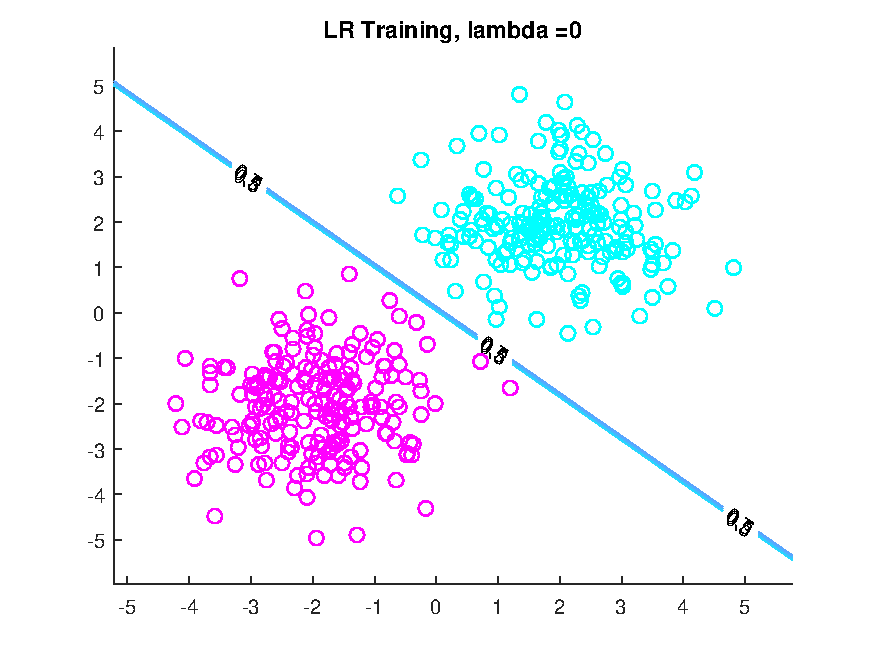
\includegraphics[scale=0.25]{hw2_1_stdev1_a_0.pdf}
	\caption{``stdev1", training}\label{fig:data_stdev1a}
    \end{subfigure}
    \quad
    \begin{subfigure}[b]{0.22\textwidth}
	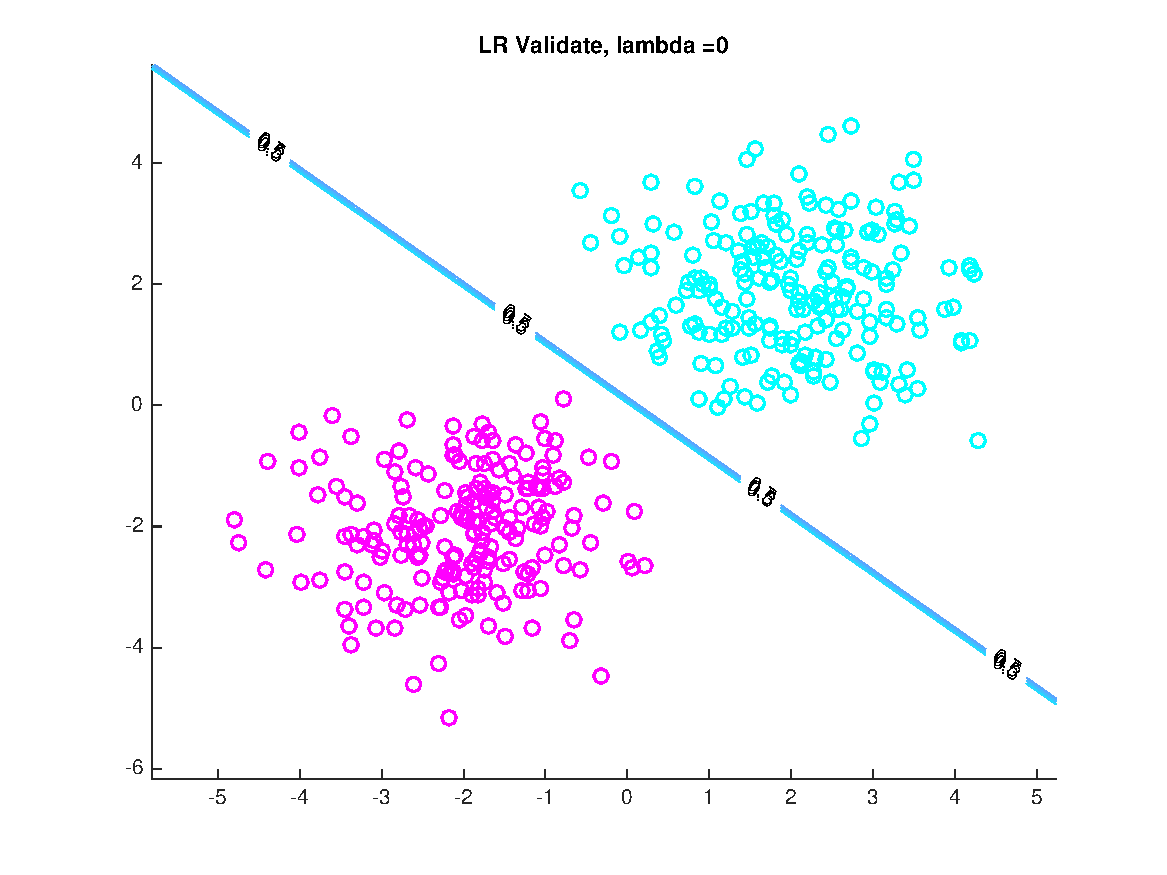
\includegraphics[scale=0.25]{hw2_1_stdev1_b_0.pdf}
	\caption{``stdev1", validation}\label{fig:data_stdev1b}
    \end{subfigure}
    \begin{subfigure}[b]{0.22\textwidth}
	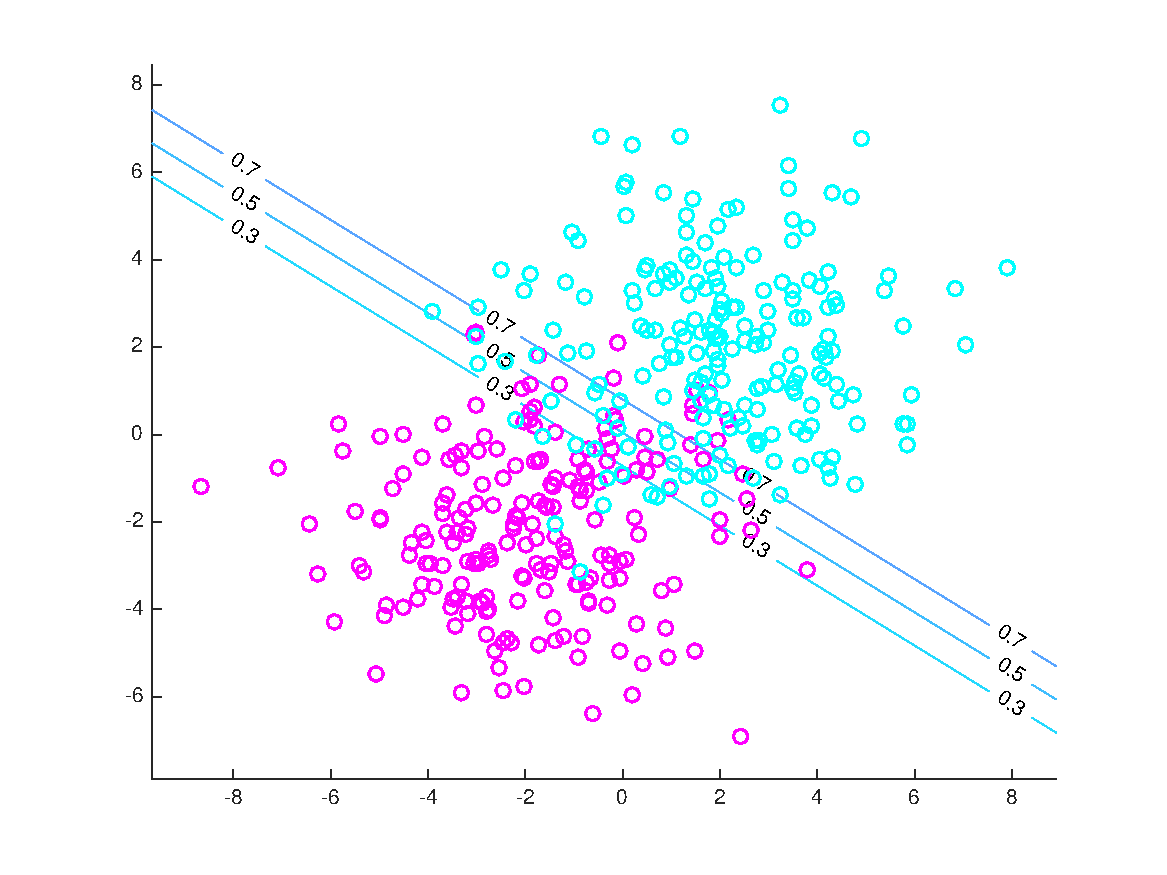
\includegraphics[scale=0.25]{hw2_1_stdev2_a_0.pdf}
	\caption{``stdev2", training}\label{fig:data_stdev2a}
	\end{subfigure}
	\quad	
	\begin{subfigure}[b]{0.22\textwidth}
	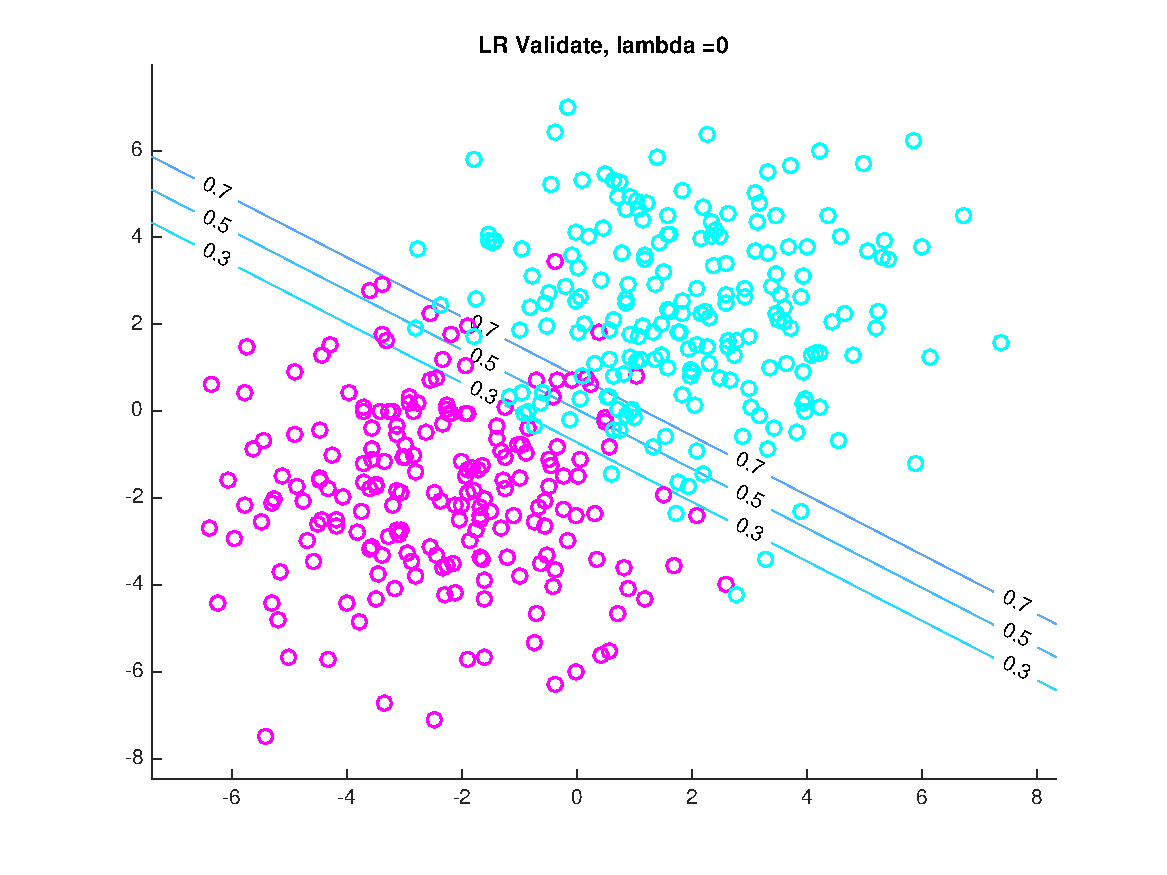
\includegraphics[scale=0.25]{hw2_1_stdev2_b_0.pdf}
	\caption{``stdev2", validation}\label{fig:data_stdev2b}
	\end{subfigure}
    
    \begin{subfigure}[b]{0.22\textwidth}
	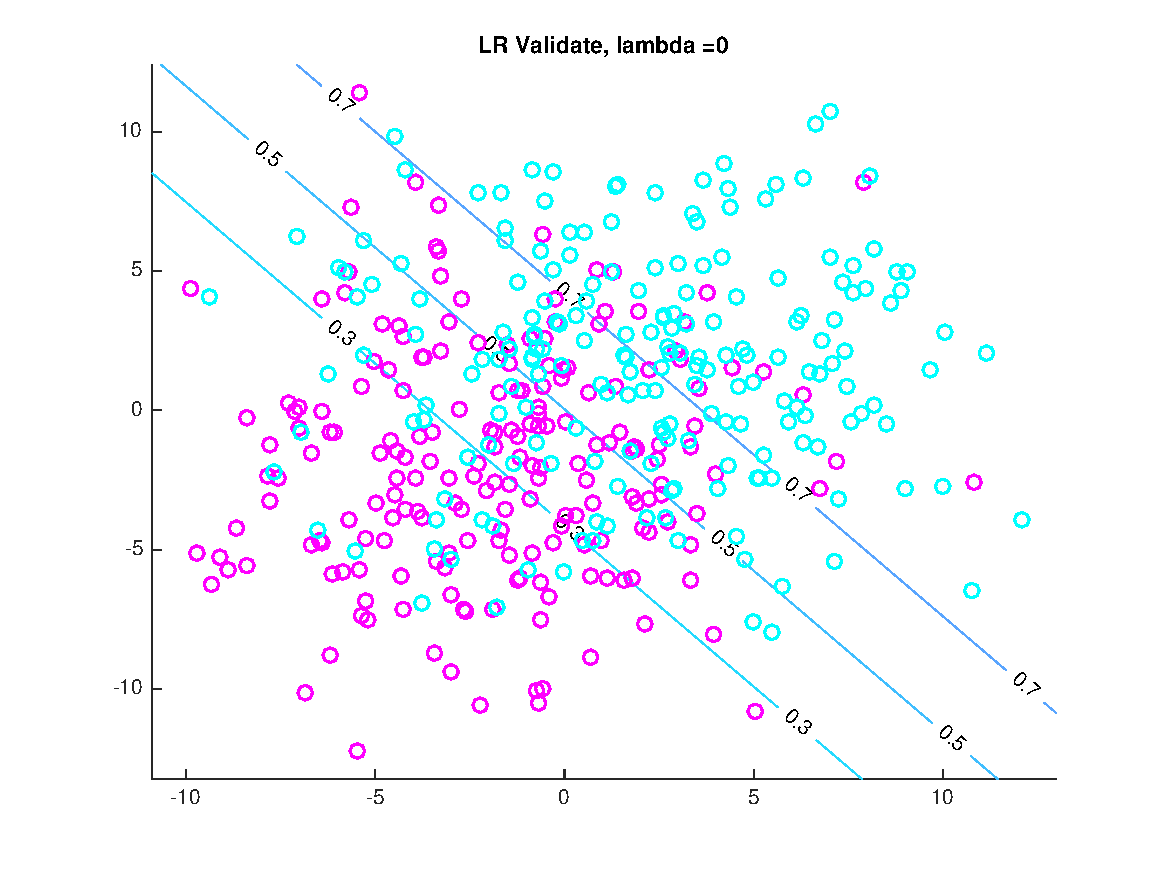
\includegraphics[scale=0.25]{hw2_1_stdev4_a_0.pdf}
	\caption{``stdev4", training}\label{fig:data_stdev4a}
    \end{subfigure}  
    \quad
    \begin{subfigure}[b]{0.22\textwidth}
	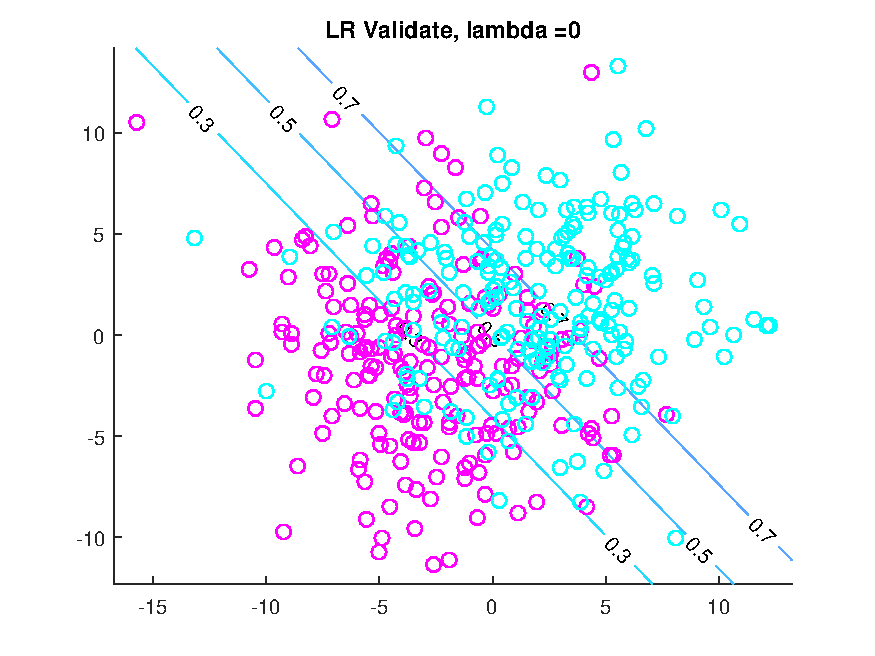
\includegraphics[scale=0.25]{hw2_1_stdev4_b_0.pdf}
	\caption{``stdev4", validation}\label{fig:data_stdev4b}
    \end{subfigure}  
    \begin{subfigure}[b]{0.22\textwidth}
	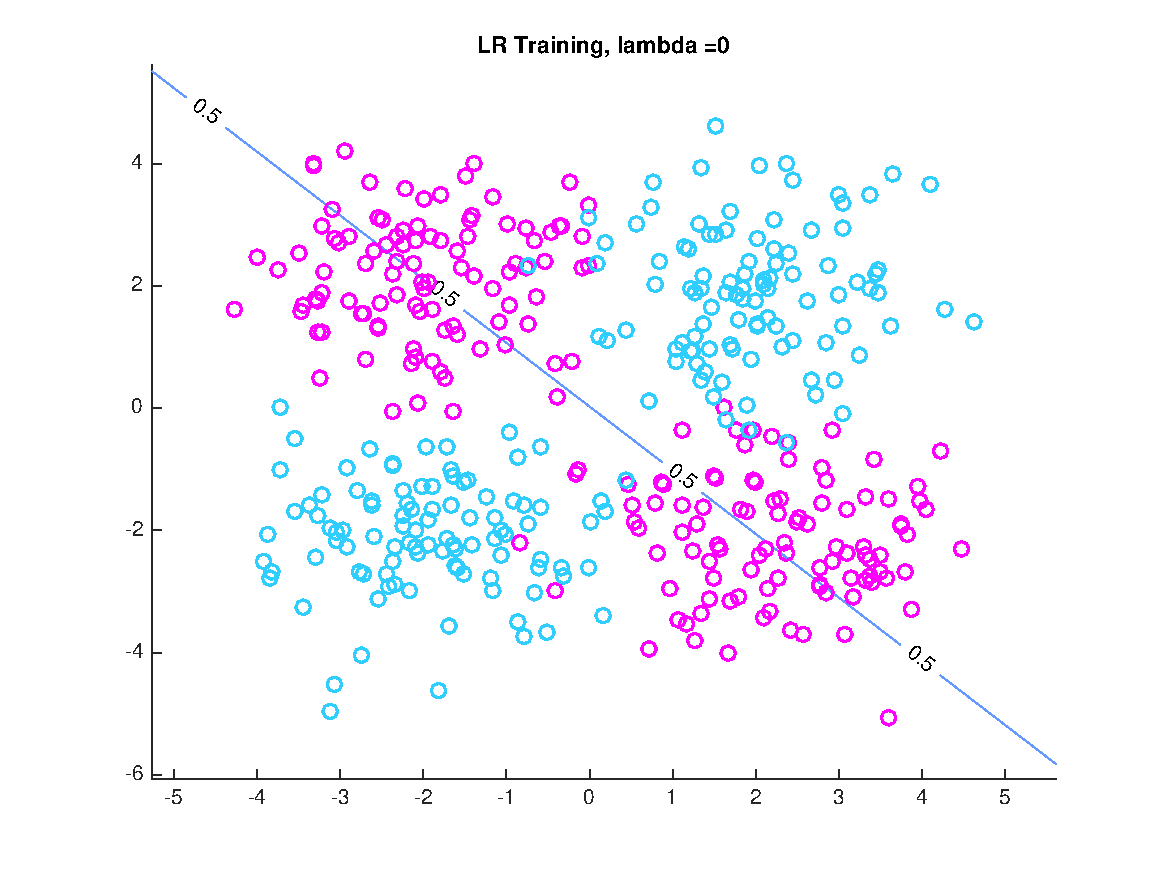
\includegraphics[scale=0.25]{hw2_1_nonsep_a_0.pdf}
	\caption{``Nonsep", training}\label{fig:data_nonsep_a}
    \end{subfigure}  
    \quad
    \begin{subfigure}[b]{0.22\textwidth}
	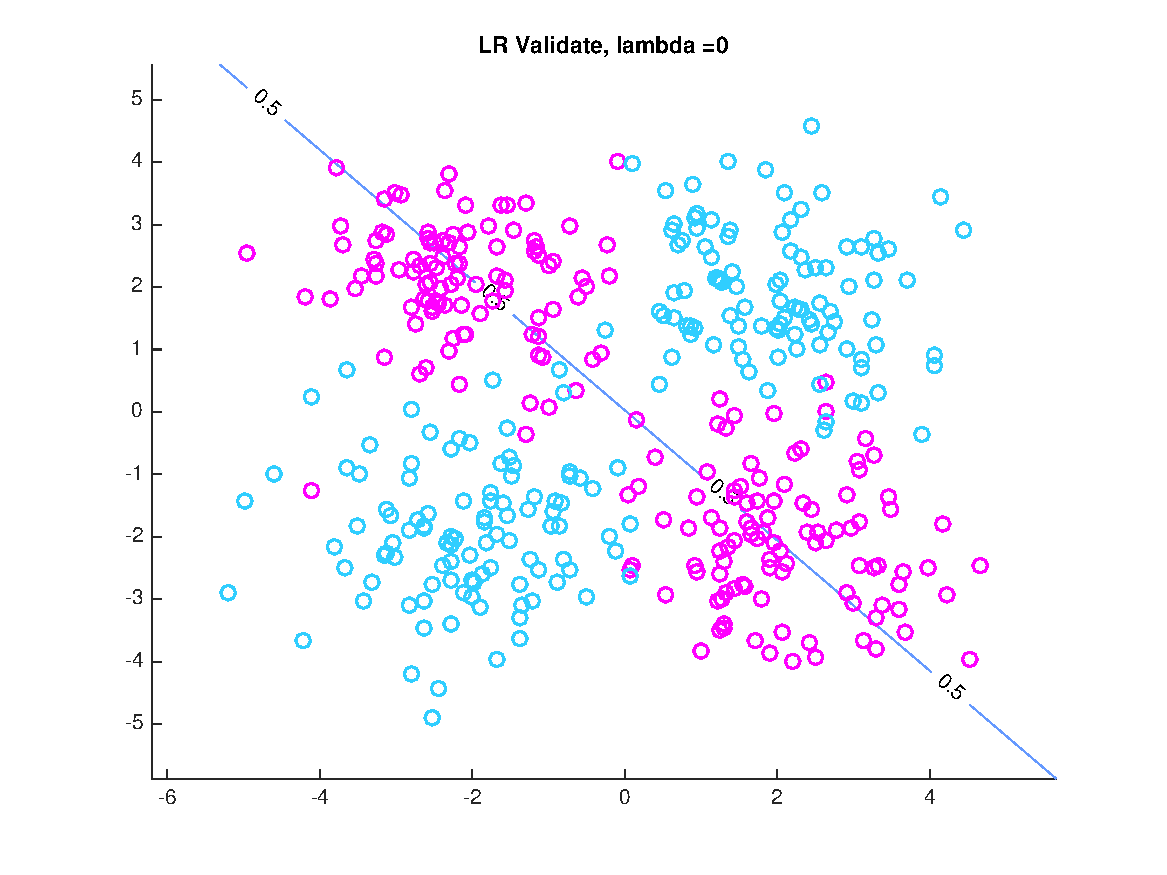
\includegraphics[scale=0.25]{hw2_1_nonsep_b_0.pdf}
	\caption{``Nonsep", validation}\label{fig:data_nonsep_b}
    \end{subfigure}  
    \caption{Plots of decision boundaries from logistic regression with $\lambda=0$ from training and validation sets.}  \label{fig:LR_plots}  
\end{figure}


\subsection{Performance on data with positive $\lambda$}
Similarly, we run logistic regression with other values of $\lambda$. As demonstrated in Figure \ref{fig:LR_plots_100}, with higher values of $\lambda$, the decision boundary is flatter, especially in more separable data. The training accuracy is lower, and the validation accuracy typically increases (or stays the same) and then decreases, as shown in Figure \ref{fig:LR_cv}. We use the cross-validation technique to select best value of $\lambda$ using the validation set accuracy. In particular, for the four datasets, we choose $\lambda = 0$, $\lambda = 0$, $\lambda = 100$, and $\lambda = 1000$ respectively. The corresponding accuracy in test sets are $0.9975$, $0.9250$, $0.7850$, and $0.5025$. Compared to not regularizing, the test set accuracies are slightly higher. The accuracy for the non-separable data set remains relatively constant regardless of how we regularize. 


\begin{figure}[h!]
\centering
    \begin{subfigure}[b]{0.22\textwidth}
	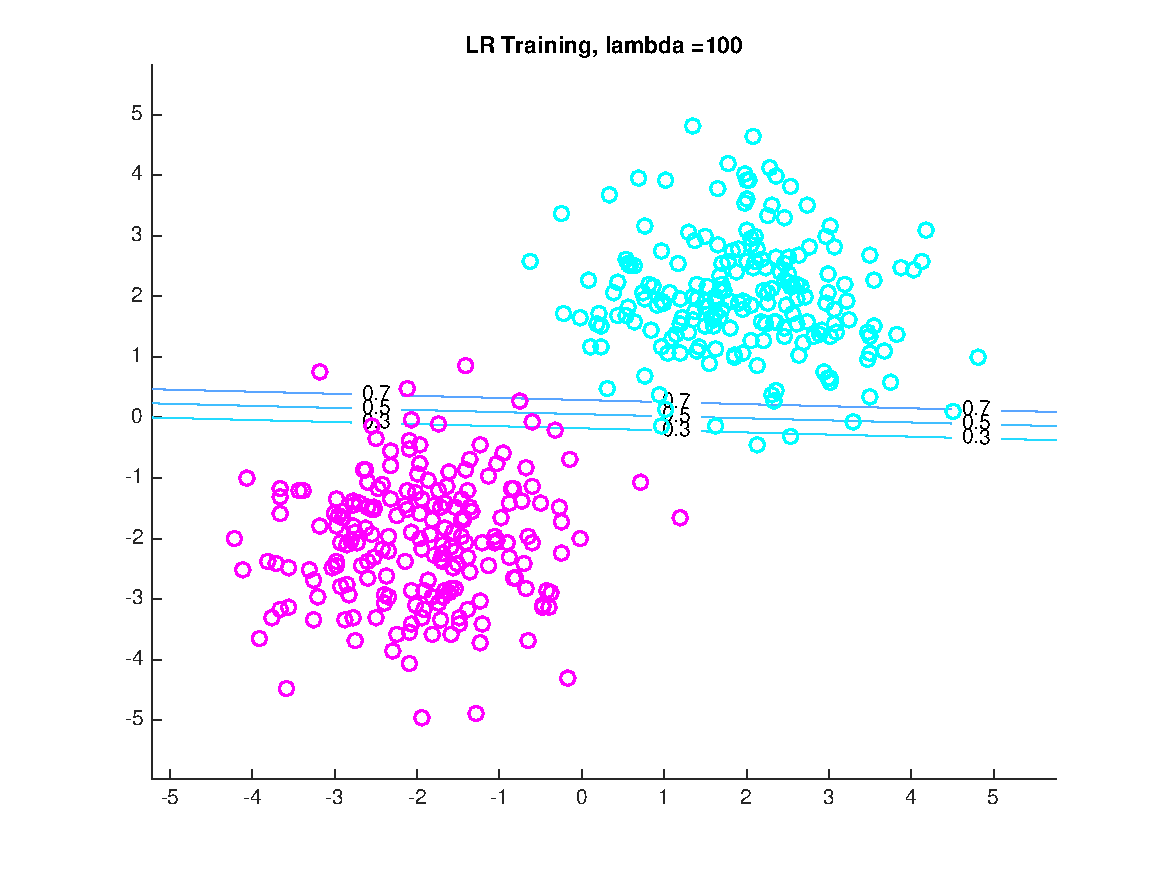
\includegraphics[scale=0.25]{hw2_1_stdev1_a_100.pdf}
	\caption{``stdev1", training}\label{fig:data_stdev1_a_100}
    \end{subfigure}
    \quad
    \begin{subfigure}[b]{0.22\textwidth}
	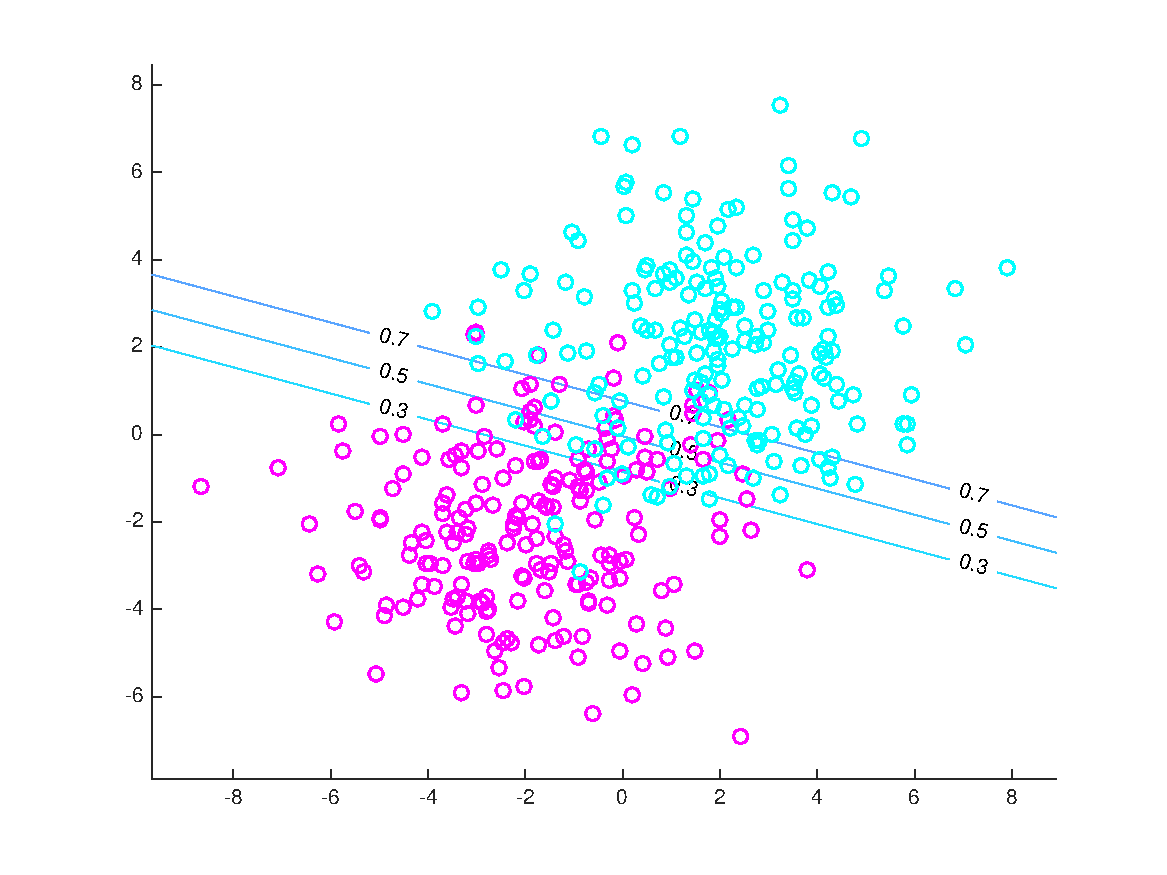
\includegraphics[scale=0.25]{hw2_1_stdev2_a_100.pdf}
	\caption{``stdev2", training}\label{fig:data_stdev2_a_100}
	\end{subfigure}
	\quad	    
    \begin{subfigure}[b]{0.22\textwidth}
	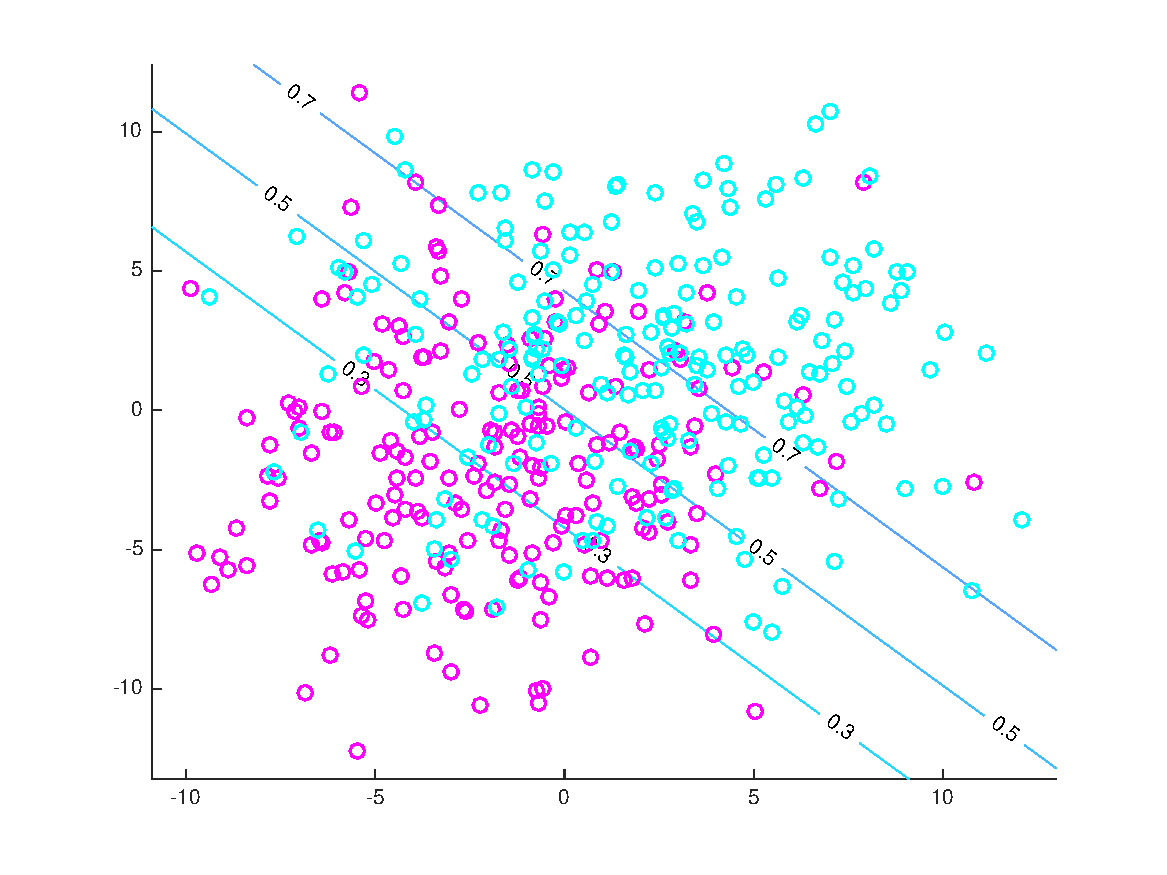
\includegraphics[scale=0.25]{hw2_1_stdev4_a_100.pdf}
	\caption{``stdev4", training}\label{fig:data_stdev4_a_100}
    \end{subfigure}  
    \quad
    \begin{subfigure}[b]{0.22\textwidth}
	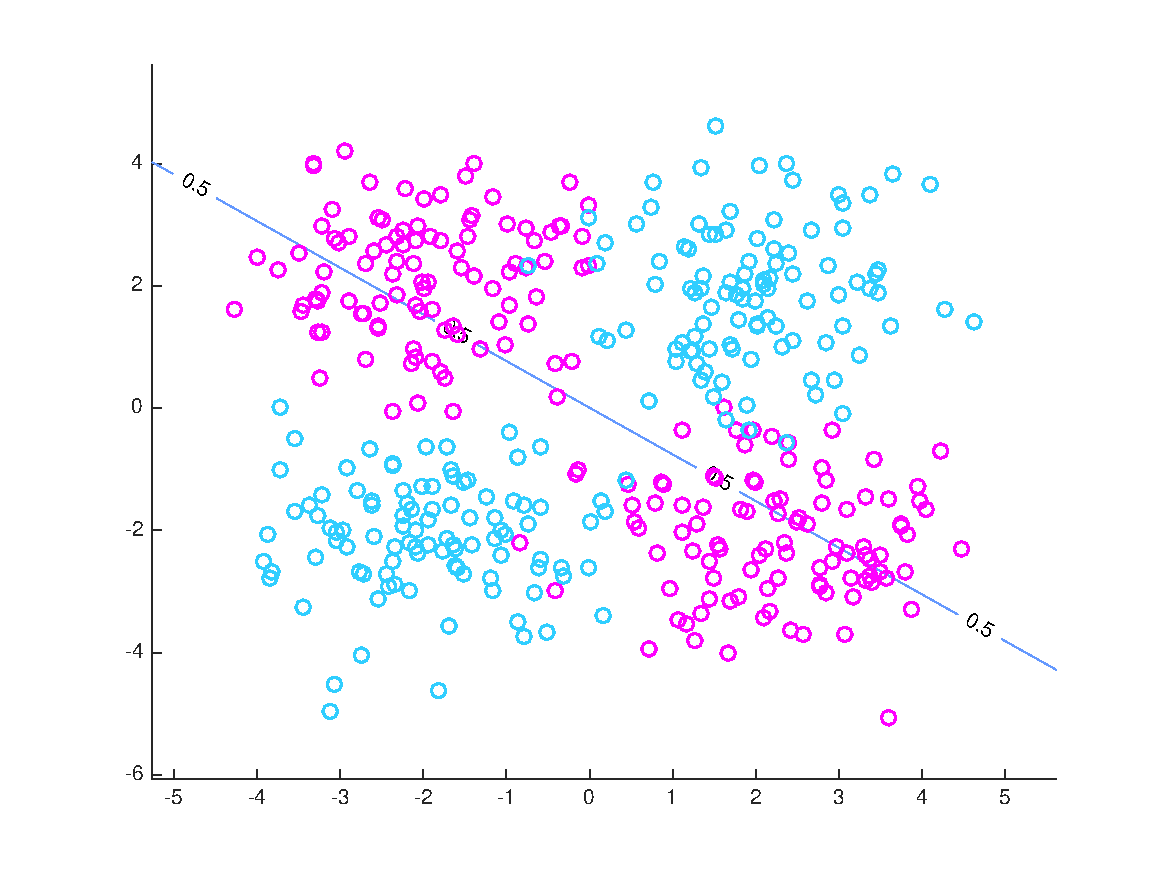
\includegraphics[scale=0.25]{hw2_1_nonsep_a_100.pdf}
	\caption{``Nonsep", training}\label{fig:data_nonsep_a_100}
    \end{subfigure}  
    \caption{Plots of decision boundaries from logistic regression with $\lambda = 100$ from four data sets.}  \label{fig:LR_plots_100}  
\end{figure}


\begin{figure}[h!]
\centering
	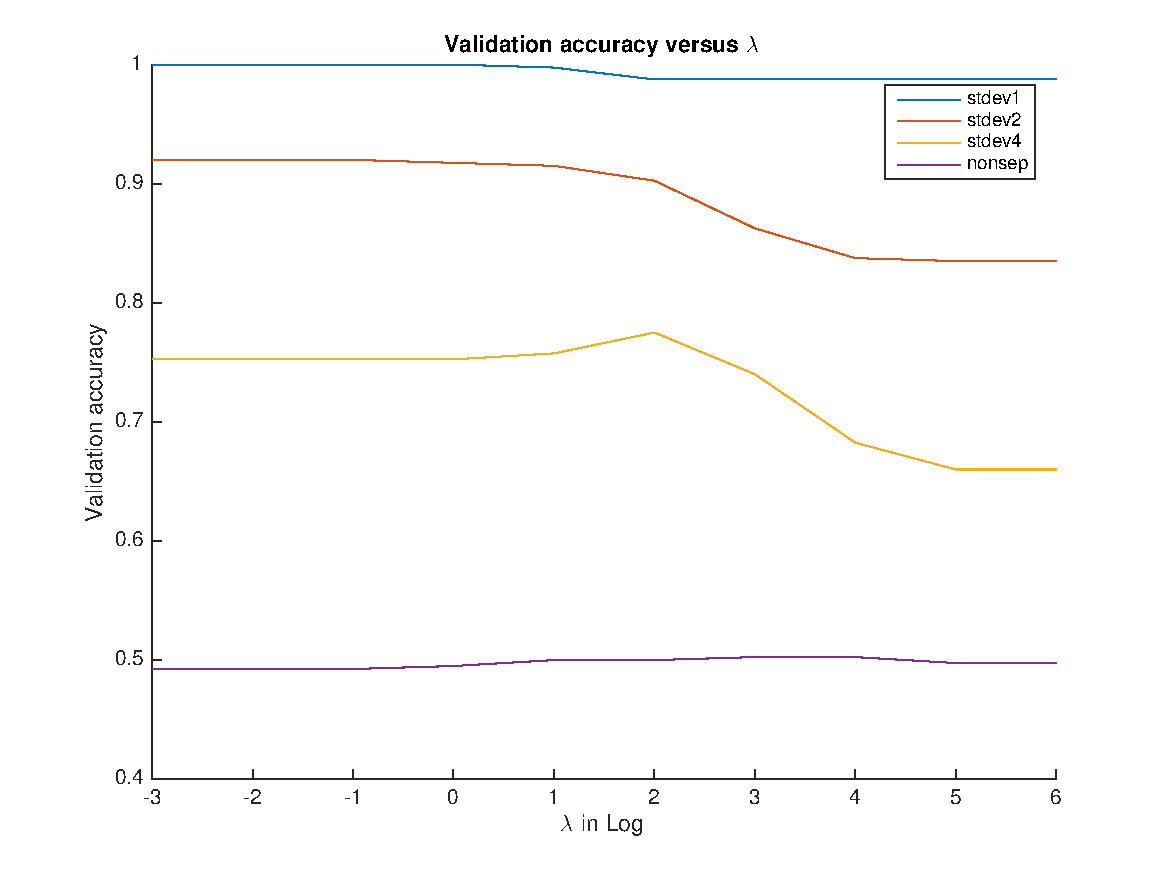
\includegraphics[scale=0.3]{hw2_1_cv.pdf}
	\caption{Cross validation error with respect to $\lambda$}\label{fig:LR_cv}
\end{figure}
	